\documentclass[12pt, dvipsnames]{beamer}
\usepackage[utf8]{inputenc}
\usepackage[T1]{fontenc}
\usepackage{lmodern}
\usetheme{}
\usecolortheme{beaver}
\setbeamertemplate{navigation symbols}{}
\setbeamertemplate{headline}{}
\setbeamertemplate{footline}{}
\setbeamercovered{transparent}
\usefonttheme{serif}
\usepackage{amsmath,amssymb,makeidx,graphicx,float,indentfirst,color,hyperref,tikz,fancyref,pgfplots,verbatim,fancyvrb,caption,subcaption,physics,longtable,mathrsfs,mathtools,xcolor,ifthen,lipsum}

\numberwithin{equation}{section}

\newcommand\blfootnote[1]{%
	\begingroup
	\renewcommand\thefootnote{}\footnote{#1}%
	\addtocounter{footnote}{-1}%
	\endgroup
}
\renewcommand{\footnotesize}{\scriptsize} 

\begin{document}
	\author{\textbf{Pritish Karmakar}\\{\footnotesize(21MS179, IISER Kolkata)}}
	\title{{On Polarization Properties of Light, Gaussian Beams and Spin-Orbit Interaction of Light}}
	\date{July 25, 2023}
\begin{frame}[plain]
	\maketitle
	\centering
	\textsl{\small Submitted to}\\
	\textbf{\small Prof. Ayan Banerjee}\\
	{\scriptsize (HOD, DPS, IISER Kolkata)}\\
	
\includegraphics[width=1.2cm]{iiserk.png}
\end{frame}
	
\begin{frame}{Topics of discussion}
	\tableofcontents
\end{frame}

\section{Polarization properties of light}

\begin{frame}
	\centering
	\alert{\huge Polarization properties of light}
	\begin{itemize}\Large
		\item<1>Jones Formalism
		\item<0>Stokes-Muller formalism
	\end{itemize}
\end{frame}

\begin{frame}{Jones Vector}\blfootnote{Wave Optics (2015)}
	Electric field of \textit{fully polarized} EM wave propagating along z-axis is given by
	\begin{align*}
		\boldsymbol{E}(\boldsymbol{r},t)=
		{\color{blue}\begin{bmatrix}
			A_x(\boldsymbol{r})e^{i\delta_x}\\
			A_y(\boldsymbol{r})e^{i\delta_y}\\
			0
		\end{bmatrix}}e^{-i(kz-\omega t)}
	\end{align*}\pause

	Define normalized \textbf{Jones vector} \textit{s.t.} $\boldsymbol{J}^\ast\:\boldsymbol{J}=1$  as
	\begin{align*}
		\boldsymbol{J}(\boldsymbol{r},t)=\frac{1}{\sqrt{A_x^2+A_y^2}}
		{\color{blue}\begin{bmatrix}
			A_x(\boldsymbol{r})e^{i\delta_x}\\
			A_y(\boldsymbol{r})e^{i\delta_y}
		\end{bmatrix}}
	\end{align*}\pause

Note that \textit{intensity}, $I= A_x^2+A_y^2 =  \boldsymbol{J}^\ast \boldsymbol{J}$
\end{frame}

\begin{frame}{Jones vector of usual polarization state}
	\begin{table}[H]
		\centering
		\begin{tabular}{ c c } 
			Polarization state & $\boldsymbol{J}$\\
			\hline
			$\ket{H}$ & $\begin{bmatrix}1\\0\end{bmatrix}$ \\ \hline
			$\ket{V}$ & $\begin{bmatrix}0\\1\end{bmatrix}$ \\ \hline
			$\ket{P}$ & $\frac{1}{\sqrt{2}}\begin{bmatrix}1\\1\end{bmatrix}$ \\ \hline
			$\ket{M}$ & $\frac{1}{\sqrt{2}}\begin{bmatrix}1\\-1\end{bmatrix}$ \\ \hline
			$\ket{L}$ & $\frac{1}{\sqrt{2}}\begin{bmatrix}1\\i\end{bmatrix}$ \\ \hline
			$\ket{R}$ & $\frac{1}{\sqrt{2}}\begin{bmatrix}1\\-i\end{bmatrix}$ \\ 
			\hline
		\end{tabular}
		\label{table:1}
	\end{table}
\end{frame}

\begin{frame}{Jones Matrix \& evolution of Jones vector}\blfootnote{Wave Optics (2015)}
	Jones matrix for an optical element be $\boldsymbol{M}$ \textit{s.t.} 
	\begin{align*}\boldsymbol{M}=
		\begin{bmatrix}
			m_{11} & m_{12}\\
			m_{21} & m_{22}
		\end{bmatrix}
	\end{align*}\pause
	If a polarized light of Jones vector $\boldsymbol{J}_{in}$ passes through that optical element then the Jones vector of output light is given by 
	\begin{align*}
		\boldsymbol{J}_{out}&=\boldsymbol{M}\;\boldsymbol{J}_{in}
	\end{align*}\pause
	\begin{itemize}
		\item Composition rule: 
		$\boldsymbol{M}=\boldsymbol{M}_1\;\boldsymbol{M}_2\dots\boldsymbol{M}_n$
		
		\item Frame rotation by $\theta$: 
		$\boldsymbol{M}_\theta = R(-\theta)\;\boldsymbol{M}\;R(\theta)$
		where $R(\theta)$ is \textit{passive rotation matrix}.
	\end{itemize}

\end{frame}

\begin{frame}{Jones matrix of usual optical element}
	\begin{longtable}[H]{ c c } 
	Optical element & $\boldsymbol{M}$\\
	\hline\endhead
	Free space & $\begin{bmatrix}
		1 & 0 \\ 
		0 & 1
	\end{bmatrix}$\\ \hline
	x-Polariser & $\begin{bmatrix}
		1 & 0 \\ 
		0 & 0
	\end{bmatrix}$\\\hline
	Right circular polariser & $\frac{1}{2}\begin{bmatrix}
		1 & i \\ 
		-i & 1
	\end{bmatrix}$\\\hline

	Linear di-attenuator & $\begin{bmatrix}
		a & 0 \\ 
		0 & b
	\end{bmatrix}$\\\hline
	\begin{tabular}{c}
		Half-wave plate\\
		with fast axis horizontal
	\end{tabular} & $\begin{bmatrix}
		1 & 0 \\ 
		0 & -1
	\end{bmatrix}$\\\hline
	\begin{tabular}{c}
		Quarter-wave plate\\
		with fast axis horizontal
	\end{tabular} & $\begin{bmatrix}
		1 & 0 \\ 
		0 & i
	\end{bmatrix}$\\\hline
	General phase retarder &  $\begin{bmatrix}
		e^{i\phi_x} & 0 \\ 
		0 & e^{i\phi_y}
	\end{bmatrix}$\\
	\hline
	\label{table:2}
\end{longtable}
\end{frame}

\begin{frame}
	\centering
	\alert{\huge Polarization properties of light}
	\begin{itemize}\Large
		\item<0>Jones Formalism
		\item<1>Stokes-Muller formalism
	\end{itemize}
\end{frame}

\begin{frame}{Coherency matrix}\blfootnote{Wave Optics (2015), Simon, B. N.; Simon, S. (2010)}
	\textit{Coherency matrix}, $\boldsymbol{C}$ defined as 
	\begin{align*}
		\boldsymbol{C}=
		\expval{\boldsymbol{E}\otimes\boldsymbol{E}^\dagger}=
			\begin{bmatrix}
				\expval{E_xE_x^\ast} & \expval{E_xE_y^\ast}\\
				\expval{E_yE_x^\ast} & \expval{E_yE_y^\ast}
			\end{bmatrix}=
		\begin{bmatrix}
			c_{xx} & c_{xy}\\
			c_{yx} & c_{yy}
		\end{bmatrix}
	\end{align*}\pause
	\begin{itemize}
		\item
		$\boldsymbol{C}=\boldsymbol{C}^\dagger$ (\alert<2>{Hermitian}).\pause
		
		\item 
		\textit{Time averaged intensity} $=\expval{E_xE_x^\ast}+\expval{E_yE_y^\ast}=\Tr(\boldsymbol{C})$\pause
		
		\item \alert<4>{Evolution of coherency matrix as 
		$\boldsymbol{C}_{out} =  \boldsymbol{M}\:\boldsymbol{C}_{in}\:\boldsymbol{M}^\dagger$} 
	\end{itemize}\pause

	Let basis set, 
	$$\left\{
	\underbrace{\begin{bmatrix}1 & 0 \\ 0 & 1\\\end{bmatrix}}_{\alert<6>{\boldsymbol{V_0}}},
	\underbrace{\begin{bmatrix}1 & 0 \\ 0 & -1\\\end{bmatrix}}_{\alert<6>{\boldsymbol{V_1}}},
	\underbrace{\begin{bmatrix}0 & 1 \\ 1 & 0\\\end{bmatrix}}_{\alert<6>{\boldsymbol{V_2}}},
	\underbrace{\begin{bmatrix}0 & i \\ -i & 0\\\end{bmatrix}}_{\alert<6>{\boldsymbol{V_3}}}
	\right\}\pause \text{ \textit{s.t.} } \boldsymbol{C} = \frac{1}{2} \sum_{i=0}^{3} S_i \alert<6>{\boldsymbol{V_i}}$$
\end{frame}


\iffalse
\begin{frame}{Stokes vector}\blfootnote{Wave Optics (2015), Hecht, E. (1970),  Simon, B. N. (2010)}
	$$\boldsymbol{C} = \frac{1}{2} \sum_{i=0}^{3} {\color{blue}S_i} \boldsymbol{V_i}\pause \longrightarrow {\color{blue}\begin{bmatrix} S_0\\ S_1\\ S_2\\S_3\end{bmatrix}}\pause = \alert<3>{\boldsymbol{S} \text{ (Stokes vector)}}$$\pause


\textbf{Measurement of Stokes parameters} \pause by passing the light through
\begin{enumerate}
	\item isotropic medium, $I_0 = S_0$\pause
	\item x-polariser, $I_1 = \frac{1}{2} (S_0+S_1)$\pause
	\item $45^\circ$-polariser, $I_2 = \frac{1}{2} (S_0+S_2)$\pause
	\item RC polariser, $I_3 = \frac{1}{2} (S_0+S_3)$
\end{enumerate}

\end{frame}
\fi


\begin{frame}[t]{Stokes vector}\blfootnote{Wave Optics (2015), Hecht, E. (1970) }
	$$\boldsymbol{C} = \frac{1}{2} \sum_{i=0}^{3} {\color{blue}S_i} \boldsymbol{V_i}\pause \longrightarrow {\color{blue}\begin{bmatrix} S_0\\ S_1\\ S_2\\S_3\end{bmatrix}}\pause = \alert<3>{\boldsymbol{S} \text{ (Stokes vector)}}$$\pause
	\alert<4,10>{$$S_1^2+S_2^2+S_3^2\le S_0^2$$}\pause
	\textbf{Degree of Polarization} \pause is the measure of polarization of light.\pause
	
	\begin{itemize}
		\item Total degree of polarization = $\sqrt{S_1^2+S_2^2+S_3^2}/S_0$\pause
		\item Degree of linear polarization = $\sqrt{S_1^2+S_2^2}/S_0$\pause
		\item Degree of circular polarization = $S_3/S_0$\pause
	\end{itemize}
	$$\alert{0\le DOP\le1}$$
	
\end{frame}

\begin{frame}{Stokes vector of usual polarization state}
	\begin{table}[H]
		\centering
		\begin{tabular}{ c c c } 
			Polarization state &  $\boldsymbol{C}$ & $\boldsymbol{S}$\\
			\hline
			$\ket{H}$ & $\begin{bmatrix}1&0\\0&0\end{bmatrix}$ & $\begin{bmatrix}1&1&0&0\end{bmatrix}^T$\\ \hline
			$\ket{V}$ & $\begin{bmatrix}0&0\\0&1\end{bmatrix}$ & $\begin{bmatrix}1&-1&0&0\end{bmatrix}^T$\\ \hline
			$\ket{P}$ & $\frac{1}{2}\begin{bmatrix}1&1\\1&1\end{bmatrix}$ & $\begin{bmatrix}1&0&1&0\end{bmatrix}^T$\\ \hline
			$\ket{M}$ & $\frac{1}{2}\begin{bmatrix}1&-1\\-1&1\end{bmatrix}$ & $\begin{bmatrix}1&0&-1&0\end{bmatrix}^T$\\ \hline
			$\ket{L}$ & $\frac{1}{2}\begin{bmatrix}1&-i\\i&1\end{bmatrix}$ & $\begin{bmatrix}1&0&0&1\end{bmatrix}^T$\\ \hline
			$\ket{R}$ & $\frac{1}{2}\begin{bmatrix}1&i\\-i&1\end{bmatrix}$ & $\begin{bmatrix}1&0&0&-1\end{bmatrix}^T$\\ \hline
			Un-polarized &  $\frac{1}{2}\begin{bmatrix}1&0\\0&1\end{bmatrix}$ & $\begin{bmatrix}1&0&0&0\end{bmatrix}^T$\\
			\hline
		\end{tabular}
	\end{table}
\end{frame}

\begin{frame}{Muller Matrix \& evolution of Stokes vector}\blfootnote{Wave Optics (2015)}
	\textit{Muller matrix} for an optical element $\boldsymbol{\mathfrak{M}}$ \textit{s.t.} 
	\begin{align*}\boldsymbol{\mathfrak{M}}=
		\begin{bmatrix}
			\mu_{11} & \cdots & \mu_{14}\\
			\vdots & \ddots & \vdots\\
			\mu_{41} & \cdots & \mu_{44}
		\end{bmatrix}
	\end{align*}\pause
	Evolution of Stokes vector as,
	$\boldsymbol{S}_{out}=\boldsymbol{\mathfrak{M}}\;\boldsymbol{S}_{in}$\pause
	\begin{itemize}
		\item Composition rule: $\boldsymbol{\mathfrak{M}}=\boldsymbol{\mathfrak{M}}_1\;\boldsymbol{\mathfrak{M}}_2 \dots {\boldsymbol{\mathfrak{M}}_n}$
		\item Frame rotation by $\theta$:
		$\boldsymbol{\mathfrak{M}}_\theta = T^{-1}(\theta)\;\boldsymbol{\mathfrak{M}}\;T(\theta)$ where $$			T(\theta)=
			\begin{bmatrix}
				1 & 0 & 0 & 0\\
				0 & \cos2\theta & \sin2\theta & 0 \\
				0 & -\sin2\theta & \cos2\theta & 0\\
				0 & 0 & 0 & 1
			\end{bmatrix}$$
	\end{itemize}
\end{frame}

\begin{frame}[t]{Poincare sphere representation}
	\begin{align*}
		{\begin{bmatrix} S_0\\ \alert<2>{S_1}\\ \alert<2>{S_2}\\ \alert<2>{S_3}\end{bmatrix} 
			\onslide<2->{\longrightarrow 
		\alert<2>{( S_1, S_2, S_3)}}}
	\end{align*}
	
	\only<3>{\centering
	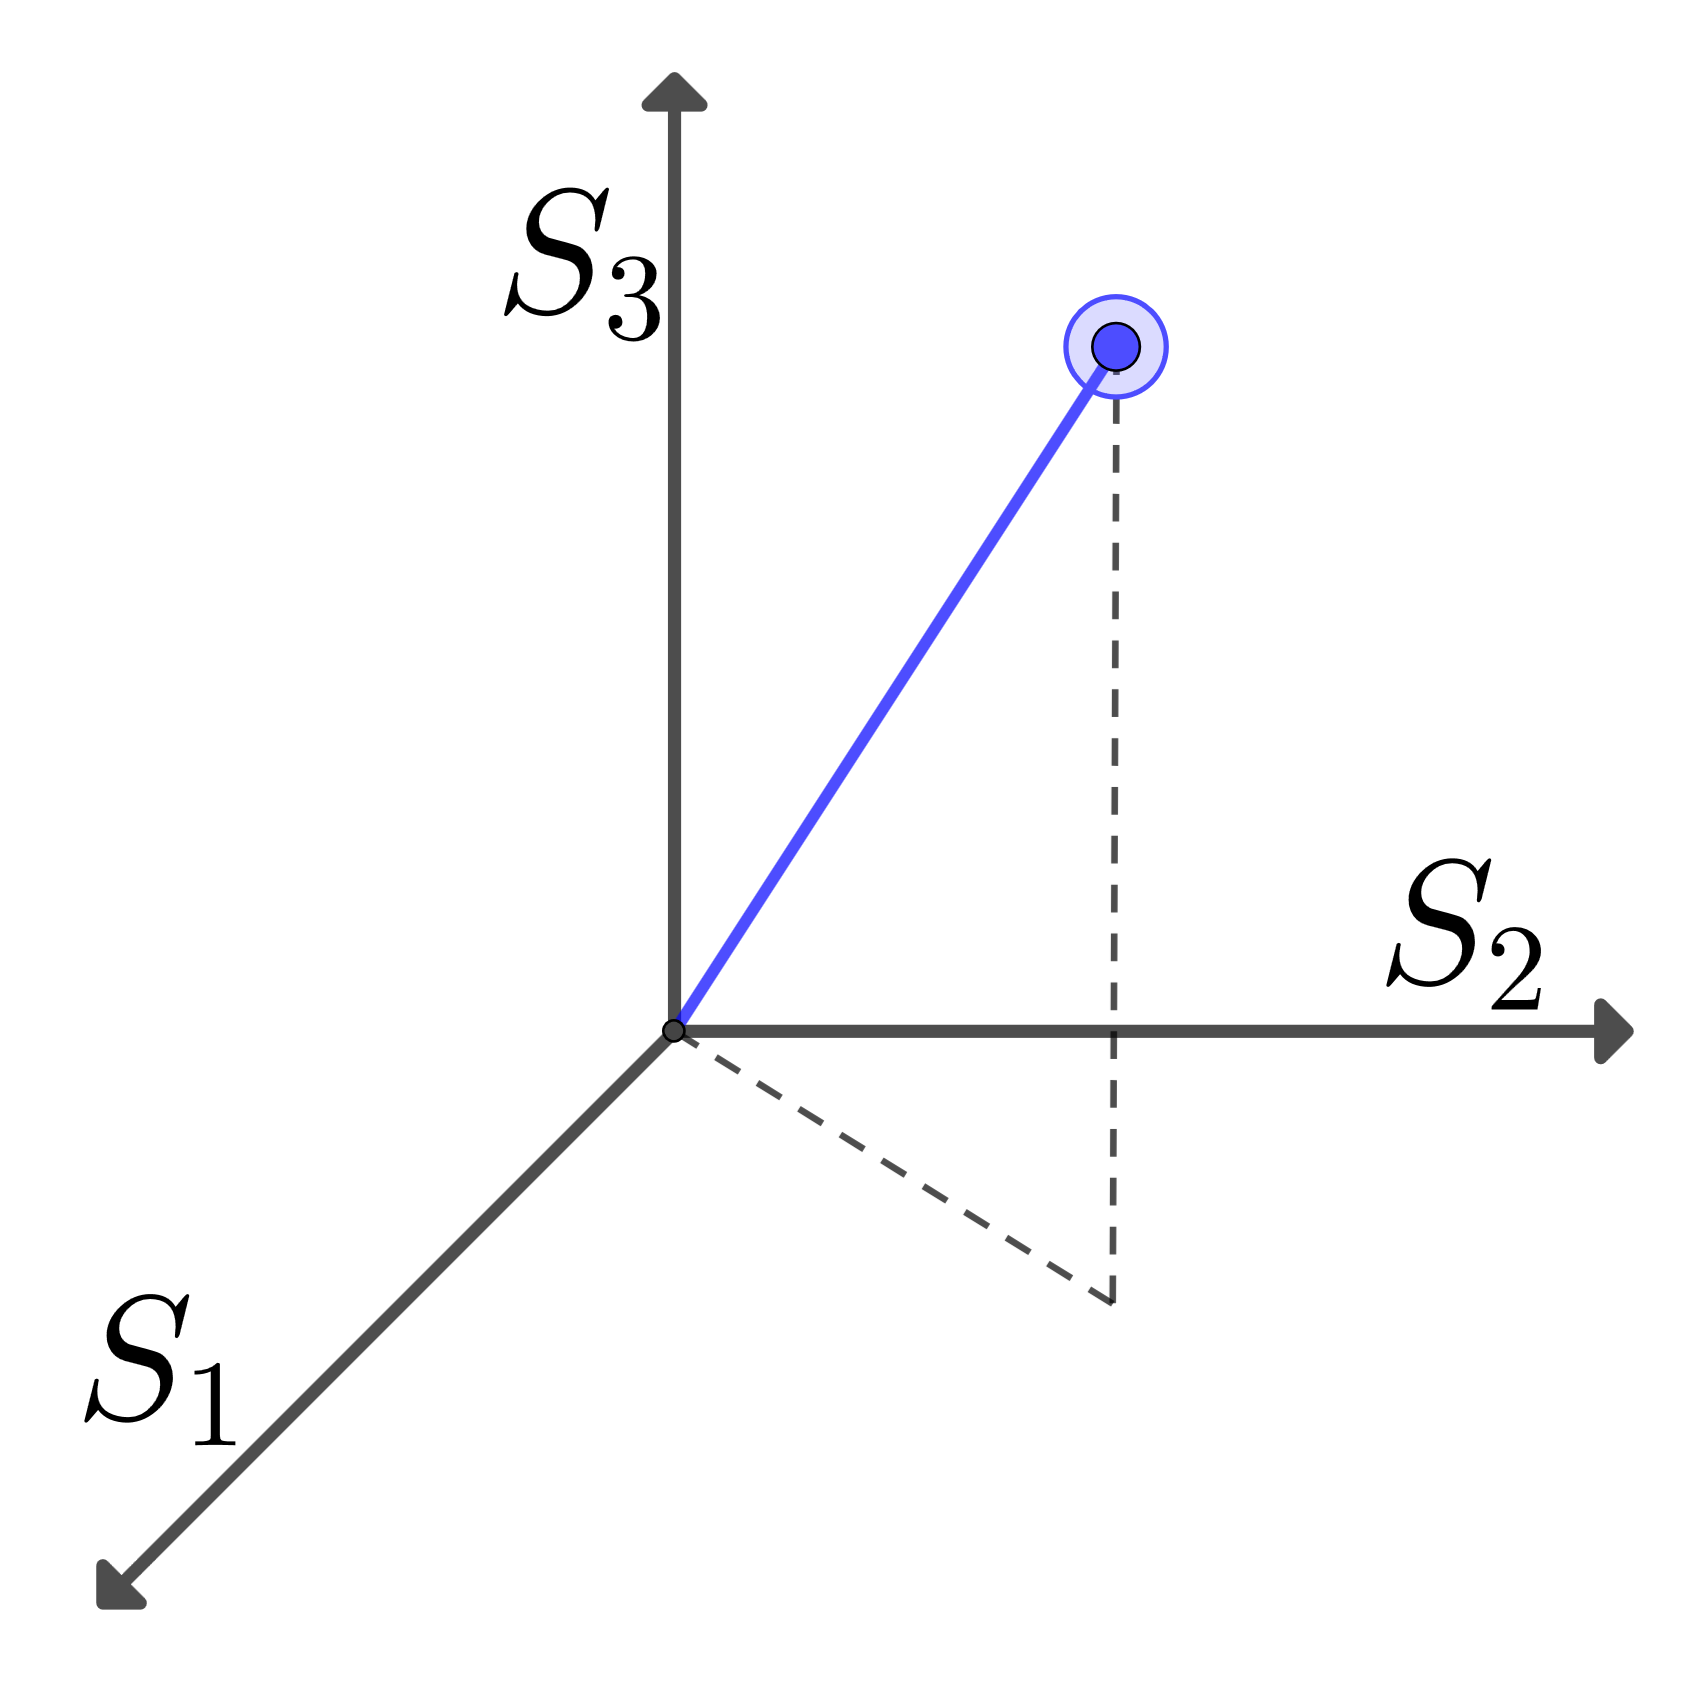
\includegraphics[width=0.4\textwidth]{poincare basic}
}
\end{frame}

\begin{frame}[t]{Poincare sphere representation}\blfootnote{Wave Optics (2015), Born, M;  Wolf, E (1999)}
	\vspace{-10pt}
	For elliptically polarized light, Stokes vector
	\begin{align*}
		\onslide<1->{\boldsymbol{S}=
		S_0
		\begin{bmatrix}
			1\\
			\cos 2\chi \cos 2\psi\\
			\cos 2\chi \sin 2\psi\\
			\sin 2\chi
		\end{bmatrix}}\onslide<2->{\longrightarrow
		\underbrace{{\color{blue}S_0}(\cos 2{\color{red}\chi} \cos 2{\color{green!45!black}\psi}, \cos 2{\color{red}\chi} \sin 2{\color{green!45!black}\psi}, \sin 2{\color{red}{\color{green!45!black}\psi}})}_{\text{On sphere of radius $S_0$}}}
	\end{align*}
\onslide<1->{where azimuth (${\color{green!45!black}\psi}$) and ellipticity (${\color{red}\chi}$) of polarization ellipse.}\\
\vspace{7pt}
	\only<3>{\begin{columns}
		\column{0.42\textwidth}
			\centering\textit{Polarization ellipse}\\
			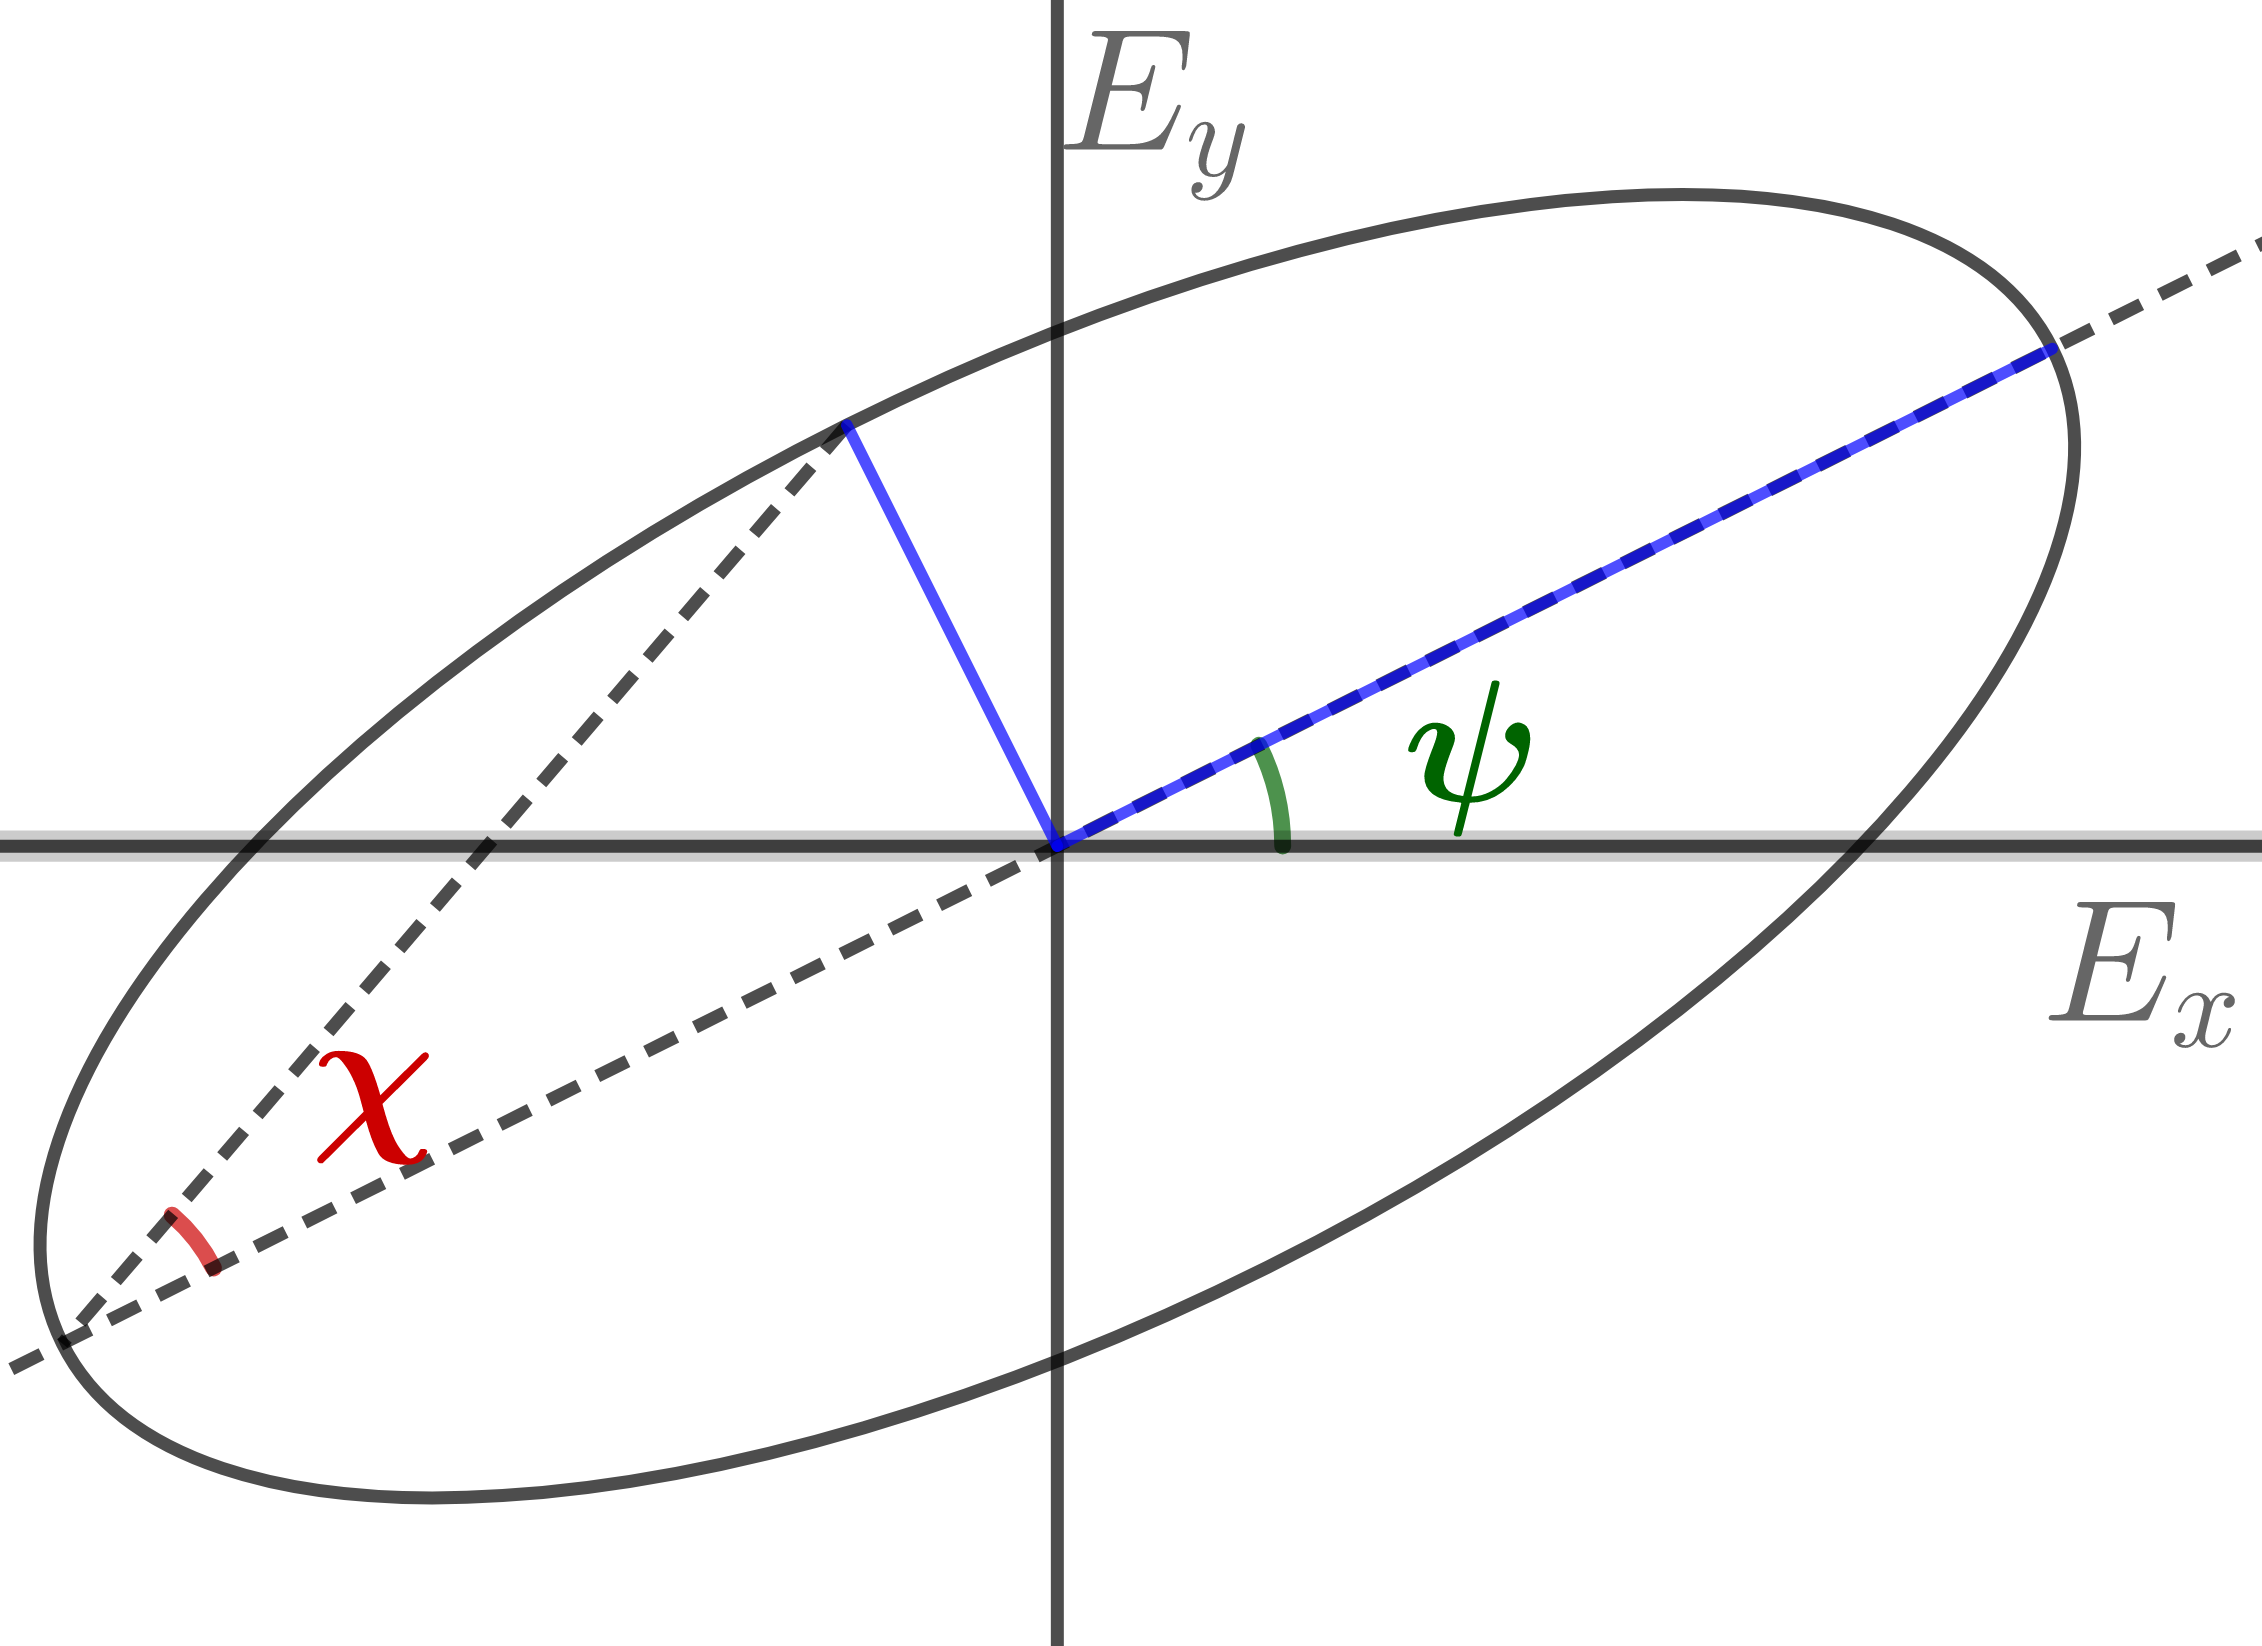
\includegraphics[width=0.96\textwidth]{ellipse beamer}
		\column{0.42\textwidth}
			\centering \textit{Poincare sphere}
			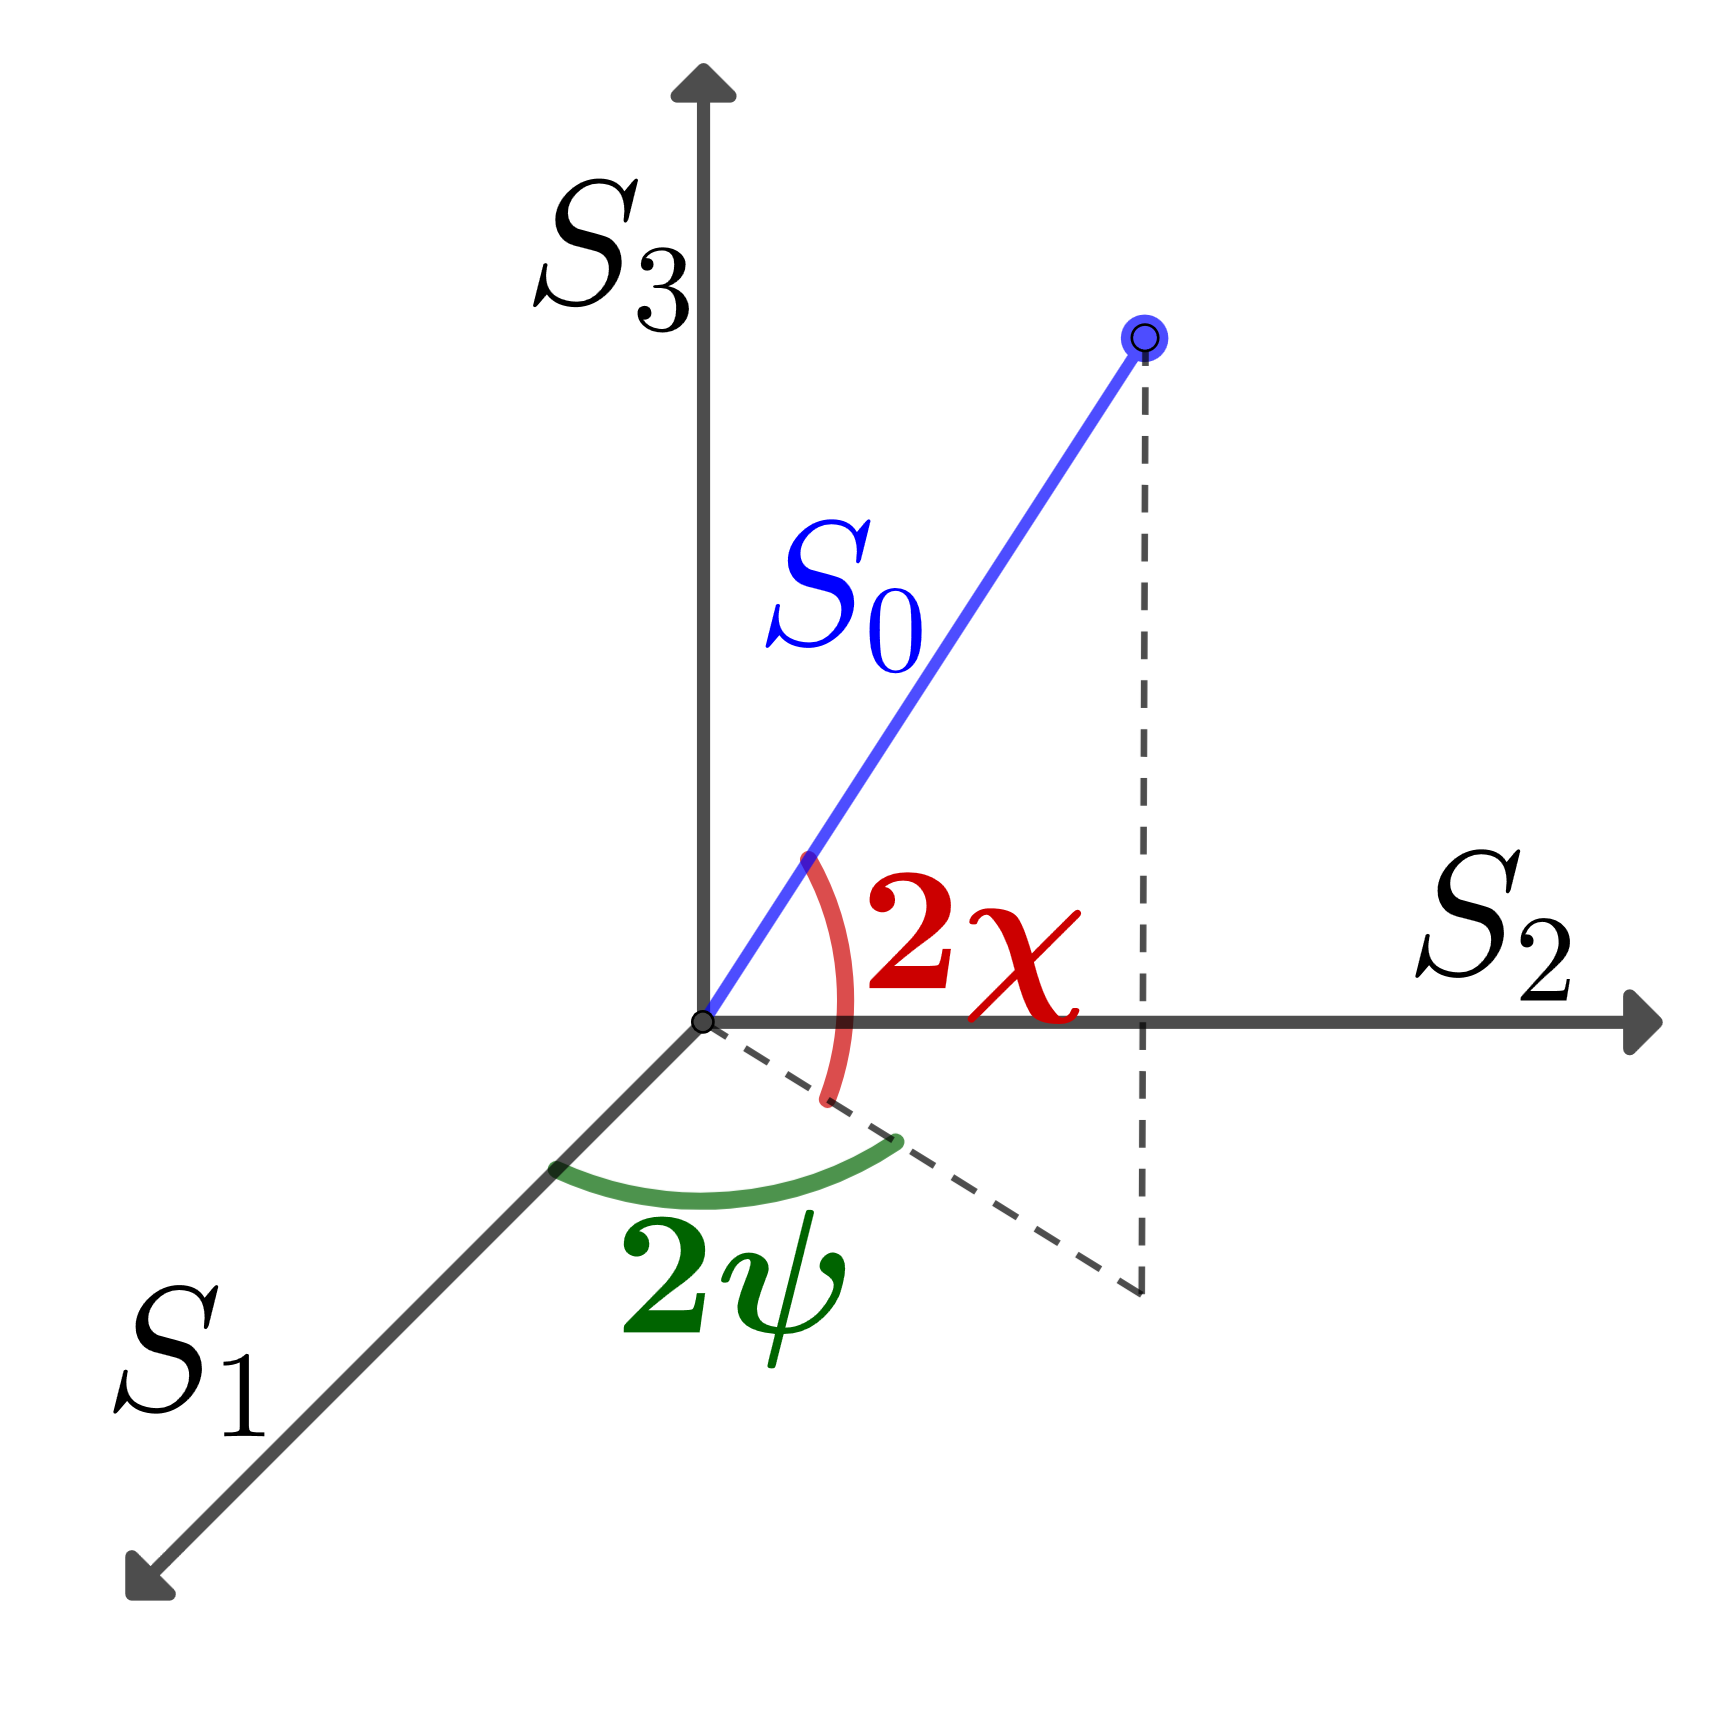
\includegraphics[width=0.72\textwidth]{poincare beamer}
	\end{columns}}

\end{frame}

\begin{frame}[t]{Poincare sphere representation}\blfootnote{Wave Optics (2015), Born, M;  Wolf, E (1999)} %2
For un-polarized light,
	\begin{align*}\boldsymbol{S}=
		S_0
		\begin{bmatrix}
			1\\
			0\\
			0\\
			0
		\end{bmatrix}\longrightarrow
		\underbrace{(0,0,0)}_{\text{At Origin}}
	\end{align*}\pause

For partially polarized light,
\begin{align*}\boldsymbol{S}=
	\begin{bmatrix}
		S_0\\
		S_1\\
		S_2\\
		S_3
	\end{bmatrix}\longrightarrow
	\underbrace{(S_1,S_2,S_3)}_{\begin{matrix}
			\text{Inside sphere \textit{s.t.}}\\
			0<S_1^2+S_2^2+S_3^2<S_0^2
		\end{matrix}}
\end{align*}

\end{frame}

\section{Gaussian Beam}

\begin{frame} %title
	\centering
	\alert{\huge Gaussian Beam and properties}
	\begin{itemize}\Large
		\item<1>Paraxial wave
		\item<0>Gaussian beam solution and properties
		\item<0>Modes of Gaussian beam
	\end{itemize}
\end{frame}

\begin{frame}{Paraxial wave}\blfootnote{Wave Optics (2015), Milonni, P.W ; Eberly, J.H.(2010)}
	\vspace{-4pt}
	Maxwell's wave equation: 
	$$\nabla^2\boldsymbol{E}(\boldsymbol{r},t) - \frac{1}{c^2} \frac{\partial^2}{\partial t^2} \boldsymbol{E}(\boldsymbol{r},t)=0$$\pause
	Paraxial beam propagating predominantly in $z$-direction, $$\boldsymbol{E}(x,y,z,t)= \boldsymbol{\psi}(x,y,z) e^{i(\omega t-kz)}$$\pause
	and taking slowly varying amplitude approx. \textit{i.e.}  $$\left|\frac{\partial^2\boldsymbol{\psi}}{\partial z^2}\right|\ll k \left|\frac{\partial\boldsymbol{\psi}}{\partial z}\right| \ll
	k^2\left|\boldsymbol{\psi}\right|$$\pause
	\textbf{Paraxial wave equation}:
	$${\color{blue}\frac{\partial^2\boldsymbol{\psi}}{\partial x^2}+\frac{\partial^2\boldsymbol{\psi}}{\partial y^2} -2ik \frac{\partial\boldsymbol{\psi}}{\partial r}=0}$$\pause
	One of the solutions is \alert{\Large Gaussian beam}.\vspace{6pt}
\end{frame}

\begin{frame}%title
	\centering
	\alert{\huge Gaussian Beam}
	\begin{itemize}\Large
		\item<0>Paraxial wave
		\item<1>Gaussian beam solution and properties
		\item<0>Modes of Gaussian beam
	\end{itemize}
\end{frame}

\begin{frame}[t]{Gaussian beam solution } \blfootnote{Milonni, P.W (2010), Kogelnik, H. (1966), \href{https://www.youtube.com/playlist?list=PLyWzPf87clvEb8T3Xf30tMaUqdbVchrNY}{ECE 4300- Cornell}}
	\vspace{-16pt}
	$$\text{Ansatz: }\psi(\boldsymbol{r},z)= A \exp\left[-i\left(p(z) + \frac{kr^2}{2q(z)}\right)\right]$$\pause
	$$\psi(\boldsymbol{r},z)=A
	\only{\left(\frac{w_0}{w(z)}\right)}
	\exp(
	{\tan[-1](\frac{z}{z_0})}\;
	{-\;i\frac{kr^2}{2R(z)}}\;
	{-\;\frac{r^2}{w^2(z)}}
	)$$\pause
	
	\only<3>{\vspace{10pt}{\begin{columns}
				\column{0.5\textwidth}\centering \textit{Electric field}
				\includegraphics[width=\linewidth]{"rad of cur beamer"}
				\column{0.5\textwidth}\centering \textit{Intensity}
				\includegraphics[width=\linewidth]{"intensity_var beamer"}
	\end{columns}}}
\end{frame}

\begin{frame}[t]{Gaussian beam properties}\blfootnote{Milonni, P.W (2010), Kogelnik, H. (1966), \href{https://www.youtube.com/playlist?list=PLyWzPf87clvEb8T3Xf30tMaUqdbVchrNY}{ECE 4300- Cornell}}%1
	\vspace{-16pt} 
	$$\psi(\boldsymbol{r},z)=A
	{\underbrace{\left(\frac{\alert{w_0}}{w(z)}\right)}_{\text{term I}}}
	\exp(
	{i\tan[-1](\frac{z}{z_0})}\;
	{-i\frac{kr^2}{2R(z)}}\;
	{-\frac{r^2}{w^2(z)}}
	)$$
{Term I related to \textbf{spreading of beam}.\\\vspace{5pt}\pause
	\begin{columns}
	\column{0.4\textwidth}
	$w\rightarrow$ Physical radius\\\pause
	{\color{red}$w_0\rightarrow$ Beam waist}\pause
	$$w(z)= w_0\sqrt{1+\left(\frac{z}{\alert<5->{z_0}}\right)^2}$$\pause
	\alert<5->{$z_0\rightarrow$ Rayleigh length}
	$$ \alert<5->{z_0} = \frac{\pi w_0^2}{\lambda}$$ 
	
	
	\column{0.5\textwidth}\only<2->{\includegraphics[width=\linewidth]{"beam waist beamer"}}
\end{columns}}

\end{frame}

\begin{frame}[t]{Gaussian beam properties}\blfootnote{Milonni, P.W (2010), Kogelnik, H. (1966), \href{https://www.youtube.com/playlist?list=PLyWzPf87clvEb8T3Xf30tMaUqdbVchrNY}{ECE 4300- Cornell}}%2
	\vspace{-16pt} 
	$$\psi(\boldsymbol{r},z)=A
	{\left(\frac{w_0}{w(z)}\right)}
	\exp(
	{\underbrace{i{\:}{\color{blue}\tan[-1](\frac{z}{z_0})}}_{\text{term II}}}\;
	{-i\frac{kr^2}{2R(z)}}\;
	{-\frac{r^2}{w^2(z)}}
	)$$
	
	{Term II related to \textbf{Gouy phase} ($\phi_G$).\\\pause
		\begin{columns}
			\column{0.4\textwidth}
			{\color{blue}$$\phi_G = \tan[-1](\frac{z}{z_0})$$}\pause
			\column{0.5\textwidth}\visible<3->{\includegraphics[width=0.9\linewidth]{"gouy beamer"}}
	\end{columns}}
\end{frame}

\begin{frame}[t]{Gaussian beam properties}\blfootnote{Milonni, P.W (2010), Kogelnik, H. (1966), \href{https://www.youtube.com/playlist?list=PLyWzPf87clvEb8T3Xf30tMaUqdbVchrNY}{ECE 4300- Cornell}}%3
	\vspace{-16pt} 
	$$\psi(\boldsymbol{r},z)=A
	{\left(\frac{w_0}{w(z)}\right)}
	\exp(
	{i\tan[-1](\frac{z}{z_0})}\;
	{\underbrace{-i\frac{kr^2}{2{\color{blue}R(z)}}}_{\text{term III}}}\;
	{-\frac{r^2}{w^2(z)}}
	)$$
	
	{Term III related to \textbf{radius of curvature} ($R$) of beam wave-front.\\\pause
		\begin{columns}
			\column{0.4\textwidth}
			{\color{blue}$$R(z)= z\left[1+\left(\frac{z_0}{z}\right)^2\right]$$} \pause
			\column{0.5\textwidth}\visible<3>{\includegraphics[width=\linewidth]{"R_vs_z beamer"}}
	\end{columns}}
\end{frame}

\begin{frame}[t]{Gaussian beam properties}\blfootnote{Milonni, P.W (2010), Kogelnik, H. (1966), \href{https://www.youtube.com/playlist?list=PLyWzPf87clvEb8T3Xf30tMaUqdbVchrNY}{ECE 4300- Cornell}}%4
	\vspace{-16pt} 
	$$\psi(\boldsymbol{r},z)=A
	{\left(\frac{w_0}{w(z)}\right)}
	\exp(
	{i\tan[-1](\frac{z}{z_0})}\;
	{-i\frac{kr^2}{2R(z)}}\;
	{\underbrace{\color{red}-\frac{r^2}{w^2(z)}}_{\text{term IV}}}
	)$$
	
	{Term IV related to \textbf{Gaussian intensity profile}.\pause
	\begin{columns}
			\column{0.4\textwidth}
				$$\color{red}I(r,z)\sim \exp(-\frac{2r^2}{w^2(z)})$$\pause
			
			\column{0.5\textwidth}
			\visible<3>{\includegraphics[width=\linewidth]{"intensity beamer"}}
	\end{columns}}
\end{frame}

\begin{frame}[t]{$q$ parameter and beam tracing}\blfootnote{Haus, H. A. (1984), \href{https://www.youtube.com/playlist?list=PLyWzPf87clvEb8T3Xf30tMaUqdbVchrNY}{ECE 4300- Cornell}}
	\vspace{-12pt}
	$$\psi(\boldsymbol{r},z)= A \exp\left[-i\left(p(z) + \frac{kr^2}{2\:\alert<1,2>{q(z)}}\right)\right]$$\pause
	$\alert<2>{q(z)}$ $\longrightarrow$ characteristic of a beam if $\lambda$ known.\pause
	\begin{align*}
		q(z) &= z + i\:\color{blue}z_0\\
		\frac{1}{q(z)} &= \frac{1}{\color{blue}R(z)} - i\: \frac{\lambda}{\pi\: \color{blue}w^2(z)}
	\end{align*}\pause

\begin{align*}\onslide<4->{{\color{red}q_{in}}\longrightarrow
	\underbrace{\boxed{\color{violet}{\begin{bmatrix}
		A&B\\
		C&D
	\end{bmatrix}}}}_{\begin{matrix}\text{Optical}\\ \text{element} \end{matrix}}
	\longrightarrow {\color{red}q_{out}}} \onslide<5>{= \frac{{\color{violet}A} {\color{red}q_{in}}+{\color{violet}B}}{{\color{violet}C} {\color{red}q_{in}}+ {\color{violet}D}}}
\end{align*}
\end{frame}

\begin{frame}%title
	\centering
	\alert{\huge Gaussian Beam and properties}
	\begin{itemize}\Large
		\item<0>Paraxial wave
		\item<0>Gaussian beam solution and properties
		\item<1>Modes of Gaussian beam
	\end{itemize}
\end{frame}

\begin{frame}[c]{Hermite-Gaussian mode}\blfootnote{Milonni, P.W (2010), Kogelnik, H. (1966)}
	\begin{align*}
		\psi_{m,n}(\boldsymbol{r},z)=& A \left(\frac{w_0}{w(z)}\right) H_m\left(\frac{\sqrt{2} x}{w(z)}\right) H_n\left(\frac{\sqrt{2} y}{w(z)}\right)\exp( -\frac{r^2}{w^2(z)}) \cdot\nonumber\\ 
		&\exp( i\:(m+n+1)\tan[-1](\frac{z}{z_0}) -i\frac{kr^2}{2R(z)})
	\end{align*}\pause
	$m,n=0\;\Rightarrow\;\psi=$ \alert{Gaussian}
\end{frame}

\begin{frame}[t]{Hermite-Gaussian Intensity profile}
	\begin{figure}
		\foreach \n in {0,1,2,3}{
			\foreach \m in {0,1,2}{
				\ifthenelse{\n<3}{
					\begin{subfigure}[htbp]{0.3\textwidth}
						\centering
						\includegraphics[width=0.8\textwidth]{intensity_hg\n\m}
						\caption{$TEM_{\n\m}$}
						%\label{fig:hg\n\m}
					\end{subfigure}
					\hfill
				}
			}
		}
	\end{figure}
\end{frame}

\begin{frame}[t]{Laguerre-Gaussian mode}\blfootnote{Milonni, P.W (2010), Kogelnik, H. (1966), Bliokh, K. Y.; Rodríguez-Fortuño, F. J. (2015)}
	\begin{align*}
		\psi_{p,l}(r,\phi,z)=&A\:\frac{w_0}{w(z)} 	\left[\frac{r\sqrt{2}}{w(z)}\right]^{|l|} L_p^{|l|}\left(\frac{2r^2}{w^2(z)}\right)\exp(-\frac{r^2}{w^2(z)}) \cdot\nonumber\\ &\exp(\only<1,2>{-il\phi}\only<3>{{\color{blue}-il\phi}}+i(2p+l+1)\tan[-1](\frac{z}{z_0})-i\frac{kr^2}{2R(z)}) 
	\end{align*}\pause
	\only<1,2>{$l,p=0\;\Rightarrow\;\psi=$ \alert{Gaussian}}\pause
	\begin{columns}
		\column{0.5\textwidth}
		$\color{blue}\exp(-il\phi)\longrightarrow$ Helical phase\\ \hspace{75pt}(carries OAM)
		
		\column{0.5\textwidth}\visible<3->{\centering \textit{Helical phase front}\\\vspace{3mm} 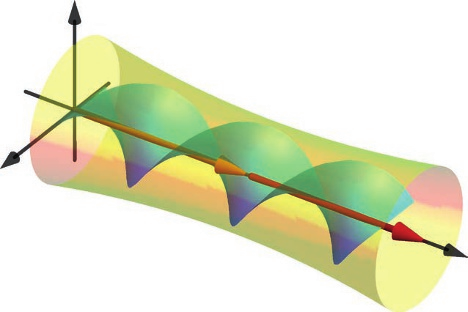
\includegraphics[width=0.7\textwidth]{ioam}}
	\end{columns}
\end{frame}

\begin{frame}[t]{Laguerre-Gaussian Intensity profile}
	\begin{figure}[t]
		\foreach \n in {0,1,2,3}{
			\foreach \m in {0,1,2}{
				\ifthenelse{\n<3}{
					\begin{subfigure}[htbp]{0.3\textwidth}
						\centering
						\includegraphics[width=0.8\textwidth]{intensity_lg\n\m}
						\caption{$p=\n,|l|=\m$}
						%\label{fig:hg\n\m}
					\end{subfigure}
					\hfill
				}
			}
		}
	\end{figure}
\end{frame}

\begin{frame}{Laguerre-Gaussian Phase profile}
	\begin{figure}
		\foreach \n in {0,1,2,3}{
			\foreach \m in {0,1,2}{
				\ifthenelse{\n<3}{
					\begin{subfigure}[htbp]{0.3\textwidth}
						\centering
						\includegraphics[width=0.8\textwidth]{phase_lg\n\m}
						\caption{$p=\n,l=\m$}
						%\label{fig:hg\n\m}
					\end{subfigure}
					\hfill
					}
				}
			}
		\end{figure}
\end{frame}

\section{Spin-orbit interaction of light}

\begin{frame} %title
	\centering
	\alert{\huge Spin-orbit interaction}
	\begin{itemize}\Large
		\item<1>Momentum of Light
		\item<0>Geometric phase of light
		\item<0>SOI in anisotropic medium
	\end{itemize}
\end{frame}

\begin{frame}{Momentum of light}
	\begin{center}
		\boxed{\text{Momentum}}\vspace{-4mm}\pause
		$$\swarrow\hspace{2cm}\searrow$$\\\vspace{-4mm}\pause
		\boxed{\text{Linear Momentum}}\hspace{1cm}\boxed{\alert<4>{\text{Angular Momentum}}}\\ \vspace{-8mm}\pause
		$$\hspace{5cm}\swarrow\hspace{1.5cm}\searrow$$\\\vspace{-4mm}\pause
		\hspace{5cm}\boxed{\alert{\text{OAM}}}\hspace{1cm}\boxed{\alert{\text{SAM}}}\\\vspace{1cm}
		\alert{\centering (For paraxial beam only)}
		
	\end{center}
\end{frame}

\begin{frame}{Linear momentum of light}\blfootnote{Haus, H. A. (1984)}
	Monochromatic beam with angular frequency $\omega$ propagating in z-direction :
	$$\boldsymbol{\mathcal{E}}(\boldsymbol{r},t) = \Re{\boldsymbol{E}(\boldsymbol{r}) e^{-i(\omega t-kz )}}$$
	$$\boldsymbol{\mathcal{B}}(\boldsymbol{r},t) = \Re{\boldsymbol{B}(\boldsymbol{r}) e^{-i (\omega t-kz ) }}$$\pause
	
	Maxwell-Faraday law:
	$$\nabla\times\boldsymbol{E}= i\omega \boldsymbol{B} $$\pause
	
	Time-averaged linear momentum per length,
	$$\mathcal{P}_z = \frac{1}{c^2}\int d\tau\: \expval{\boldsymbol{S}}_z\pause
	=\frac{\epsilon_0}{2i\omega}\iint  dx\:dy\: \expval{\boldsymbol{E}\times (\nabla\times\boldsymbol{E})}_z$$
\end{frame}

\begin{frame}{Angular momentum of light}\blfootnote{Allen, L. (1999), Wave Optics (2015), S.J. van Enk; G. Nienhuis (1992), Cohen-Tannoudji, C., Dupont-Roc, J. (1989)}
	Time-averaged AM per length :
	$$\mathcal{J}_z=\frac{1}{c^2}\int d\tau\: [\boldsymbol{r}\times\expval{\boldsymbol{S}}]_z=\pause
	\frac{\epsilon_0}{2i\omega}\iint dx\:dy\: \left[\boldsymbol{r}\times\expval{\boldsymbol{E}\times (\nabla\times\boldsymbol{E})}\right]_z$$\pause
	For paraxial beam,
	\begin{align*}
		\mathcal{J}_z
		= &\alert<4>{\frac{\epsilon_0}{2i\omega} \iint dx\:dy\:\left[E_\xi^\ast\left(x\frac{\partial}{\partial y} - y\frac{\partial}{\partial x}\right)E_\xi\right]_{\xi=x,y}}
		\\
		&+\alert<5>{\frac{\epsilon_0}{2i\omega}\iint dx\:dy\: (E_x^\ast E_y + E_y^\ast E_x)}
	\end{align*}
	
	\begin{center}
		\only<4>{\alert{Orbital AM, $\mathcal{L}$}} 
		\only<5>{\alert{Spin AM, $\mathcal{S}$}}
	\end{center}
\end{frame}

\begin{frame}[t]{Orbital AM}\blfootnote{Allen, L. (1999), Wave Optics (2015), S.J. van Enk (1992),Berry, M. V.; Soskin, M. S. (1998)}
	\vspace{-9pt}
	$$\mathcal{L}
	= \frac{\epsilon_0}{2i\omega} \iint dx\:dy\:\left[E_\xi^\ast\left({\boldsymbol{r}}\times\nabla\right)_zE_\xi\right]_{\xi=x,y}$$\pause
	for vortex beam,
	$$\boldsymbol{E}(r,\phi)= u(r)\:\exp(-il\phi)\:\Hat{\boldsymbol{p}}$$\pause
	$$\mathcal{W}_z=\frac{\epsilon_0}{2}\iint dx\:dy\: \boldsymbol{E}^\ast\cdot\boldsymbol{E}$$\pause
	$$\frac{\mathcal{L}}{\mathcal{W}_z}  =\frac{\text{OAM}}{\text{Total energy}}\pause= \frac{l}{\omega}$$
\end{frame}

\begin{frame}[t]{Orbital AM}\blfootnote{Allen, L. (1999), Wave Optics (2015), S.J. van Enk (1992), Berry, M. V.; Soskin, M. S. (1998)}%2
	\vspace{-9pt}
	$$\mathcal{L}
	= \frac{\epsilon_0}{2i\omega} \iint dx\:dy\:\left[E_\xi^\ast\left(\alert<2>{\boldsymbol{r}}\times\nabla\right)_zE_\xi\right]_{\xi=x,y}$$\pause
	\alert<2>{OAM depends on the choice of the axis.}\pause
	$$\boldsymbol{r}\longrightarrow\boldsymbol{r'}=\boldsymbol{r}+\boldsymbol{r_0}$$\pause\vspace{-8mm}
	$$\mathcal{L}\longrightarrow\mathcal{L'}= \mathcal{L}_z + \alert<5>{\Delta\mathcal{L}}$$\pause\vspace{-8mm}
	
	\begin{center}
		\boxed{\text{OAM}}\vspace{-4mm}\pause
		$$\swarrow\hspace{2cm}\searrow$$\\\vspace{-2mm}\pause
		\boxed{\alert<8,9,10>{\text{Intrinsic}}}\hspace{1cm}\boxed{\alert<10>{\text{Extrinsic}}}
	\end{center}\pause
	\only<8,9>{\alert<8,9>{$$\Delta\mathcal{L}=0$$}\pause\vspace{-5mm}
	\alert<8,9>{$$\iint  dx\:dy\: \left[E_\xi^\ast\left(\boldsymbol{r_0}\times\nabla\right)_zE_\xi\right] = 0$$}}

	\only<10>{\alert<10>{$$\Delta\mathcal{L}\ne0$$}}
\end{frame}

\begin{frame}[t]{Spin AM}\blfootnote{Allen, L. (1999), Wave Optics (2015), S.J. van Enk (1992)}
	$$\mathcal{S}=\frac{\epsilon_0}{2i\omega}\iint dx\:dy\: \alert<2>{(E_x^\ast E_y + E_y^\ast E_x)}$$\\\pause
	\alert<2>{SAM is \textbf{intrinsic}}.\\\pause
	For vortex beam,
	$$\boldsymbol{E}(r,\phi)= u(r)\:\exp(-il\phi)\:\Hat{\boldsymbol{p}}$$\pause\vspace{-3mm}
	$$\frac{\mathcal{S}}{\mathcal{W}_z} =\frac{\text{SAM}}{\text{Total energy}} \pause = \frac{\alert<6>{\sigma}}{\omega} $$\pause
	
	$\alert<6>{\sigma=2\;\Im(p_x^\ast\: p_y)}\rightarrow$ helicity of beam\pause
	
	$$\frac{\mathcal{J}_z}{\mathcal{W}_z} = \frac{\mathcal{L}+\mathcal{S}}{\mathcal{W}_z} =\frac{\text{Total AM}}{\text{Total energy}} \pause=\frac{l+\sigma}{\omega}$$
\end{frame}

\begin{frame}{Visualisation of AM}\blfootnote{Bliokh, K. Y. (2015)}
	\begin{columns}
		\column{0.5\textwidth}
		\visible<1->{\includegraphics[width=\linewidth]{"ioam"}}\\
		\visible<2->{\includegraphics[width=\linewidth]{"eoam"}}
		
		\column{0.5\textwidth}
		\visible<3->{\includegraphics[width=\linewidth]{"sam"}}
\end{columns}
\end{frame}

\begin{frame} %title
	\centering
	\alert{\huge Spin-orbit interaction}
	\begin{itemize}\Large
		\item<0>Momentum of Light
		\item<1>Geometric phase of light
		\item<0>SOI in anisotropic medium
	\end{itemize}
\end{frame}

\begin{frame}[c]{Geometric phase}\blfootnote{Wave Optics (2015), Bliokh, K. Y. (2015)}
	\begin{center}
		\boxed{\text{Phase}}\vspace{-4mm}\pause
		$$\swarrow\hspace{1.5cm}\searrow$$\\\vspace{-2mm}\pause
		\boxed{\alert<4>{\text{Dynamical phase}}} \hspace{1cm}\boxed{\alert<5->{\text{Geometric phase}}}\\\pause
	\end{center}

		\only<4>{Associated with optical path length.}
		\only<5->{Associated with geometry of evolution.}\pause
		\visible<6>{\begin{itemize}
			{\item \alert{Spin-redirection Berry phase}}
			{\item \alert{Pancharatnam-Berry Phase}}
		\end{itemize}}
\end{frame}

\begin{frame}[t]{Spin-redirection Berry phase}\blfootnote{Wave Optics (2015), Bliokh, K. Y. (2015), \href{https://www.physics.usu.edu/Wheeler/GenRel2013/Notes/Curvature.pdf}{Parallel transport- Utah State}}
	Associated with adiabatic evolution of wave-vector.\pause \\
	\textit{e.g.,} Polarized light through a helical optic fibre.\pause
	\begin{columns}
		\column{0.5\textwidth}
		$$\boldsymbol{J}=\begin{bmatrix}
			1\\i\sigma
		\end{bmatrix}\longrightarrow\boldsymbol{J'}=\boldsymbol{J}\alert<2,3>{\exp(i \sigma\alert<4,5>{\Theta})}$$
		\only<3>{\centering \alert<3>{Helicity-dependant geometric phase}\vspace{-4mm}}
		\pause
		$$\alert{\Theta} = 2\pi(1-\cos\theta)$$\pause
		$\alert{\Theta}\rightarrow$ solid angle obtained at the apex of the cone.\pause
		\begin{align*}
			\ket{L}&\longrightarrow e^{i\Theta}\ket{L}\\
			\ket{R}&\longrightarrow e^{-i\Theta}\ket{R}
		\end{align*}
	
		\column{0.5\textwidth}
		\begin{center}
		\only<2,3>{\includegraphics[width=\linewidth]{"berry"}}
		
		\only<4->{
			\includegraphics[width=0.7\linewidth]{"k sphere beamer"}\\
			\textit{Parallel transport}}
		\end{center}
	\end{columns}
\end{frame}

\begin{frame}[t]{Pancharatnam-Berry Phase}\blfootnote{Wave Optics (2015), Chyba, T. H.; Wang, L. J. (1988)}
	Associated with cyclic evolution in Poincare sphere keeping wave-vector fixed.\pause\\ 
	\textit{e.g.,} Michelson interferometer.\\\vspace{1mm}\pause

	\begin{columns}
		\column{0.5\textwidth}
		\alert<3>{QP1}$\rightarrow$fixed (aligned at $\pi/4$)\\
		\alert<3,9>{QP2}$\rightarrow$movable (aligned at $\beta$)\pause
		\begin{align*}
			\boldsymbol{J}_A&= \ket{x}\\\pause
			\boldsymbol{J}_A &\longrightarrow \boldsymbol{J}_A'\\\pause
			\boldsymbol{J}_A'&=\ket{x}\exp(i\phi_d)\:\alert<8>{\exp(-i\:2\alert<9>{\varphi})}\pause
		\end{align*}
		$$\alert<9->{\varphi}= \beta+\pi/4$$\pause
		\onslide<8>{\alert{Pancharatnam-Berry Phase}}\pause\\
		\alert<9>{(\alert{$\varphi$} depends on QP2 alignment)}
		\column{0.5\textwidth}
			\only<2>{\centering\includegraphics[width=\linewidth]{"pb expt"}}
			\only<3->{\centering\includegraphics[width=0.8\linewidth]{"MI arm beamer"}\\\vspace{3mm}\includegraphics[width=0.8\linewidth]{"poincare-pb"}}
	\end{columns}
\end{frame}

\begin{frame} %title
	\centering
	\alert{\huge Spin-orbit interaction}
	\begin{itemize}\Large
		\item<0>Momentum of Light
		\item<0>Geometric phase of light
		\item<1>SOI in anisotropic medium
	\end{itemize}
\end{frame}

\begin{frame}{Spin-orbit interaction of light}\blfootnote{Bliokh, K. Y. (2015)}
	Three types of AM:
	\begin{itemize}
		\item<2->IOAM
		\item<3->EOAM
		\item<4->SAM
	\end{itemize}

	\onslide<5>{Inter-conversion between AM in a process represents \textbf{spin-orbit interaction} of light}
\end{frame}

\begin{frame}{SOI in homogeneous-anisotropic media} \blfootnote{Wave Optics (2015)}
	\textit{e.g.} \textbf{Quarter wave-plate}\pause
	\begin{align*}
		{\color{blue}\begin{matrix}
			\text{Circularly}\\
			\text{polarized}\\
			(\sigma=\pm1)
		\end{matrix}\longrightarrow}
		&\boxed{\begin{matrix}
			\text{Q}\\
			\text{W}\\
			\text{P}
		\end{matrix}}{\color{blue}\longrightarrow
		\begin{matrix}
			\text{Linearly}\\
			\text{polarized}\\
			(\sigma=0)
		\end{matrix}}
	\end{align*}\pause
	$\pm\hbar$ SAM per photon is transferred to the wave plate.\\\pause

	\textit{e.g.} \textbf{Half wave-plate}\pause
	\begin{align*}
		{\color{blue}\begin{matrix}
				\text{Circularly}\\
				\text{polarized}\\
				(\sigma=\pm1)
			\end{matrix}\longrightarrow}
		&\boxed{\begin{matrix}
				\text{H}\\
				\text{W}\\
				\text{P}
		\end{matrix}}{\color{blue}\longrightarrow
			\begin{matrix}
				\text{Circularly}\\
				\text{polarized}\\
				(\sigma=\mp1)
		\end{matrix}}
	\end{align*}\pause
	$\pm2\hbar$ SAM per photon is transferred to the wave plate and spin is flipped.
\end{frame}

\begin{frame}[t]{SOI in inhomogeneous-anisotropic media} 
	e.g. \textbf{q-plate}\\\pause
	Inhomogeneous orientation of the fast axis varying with azimuth ($\phi$).\\
	
	\begin{columns}
		\column{0.5\textwidth}
		\only<3>{$$\alpha(\phi)=q\phi+\alpha_0$$}
		\column{0.5\textwidth}
		\begin{center}
			\only<3>{\includegraphics[width=\linewidth]{"q-plate"}}
		\end{center}
	\end{columns}
\end{frame}

\begin{frame}[t]{q-plate}\blfootnote{Marrucci, L.; Manzo, C. (2006)}
	\begin{figure}[H]
		\begin{subfigure}[H]{0.35\textwidth}
			\centering
			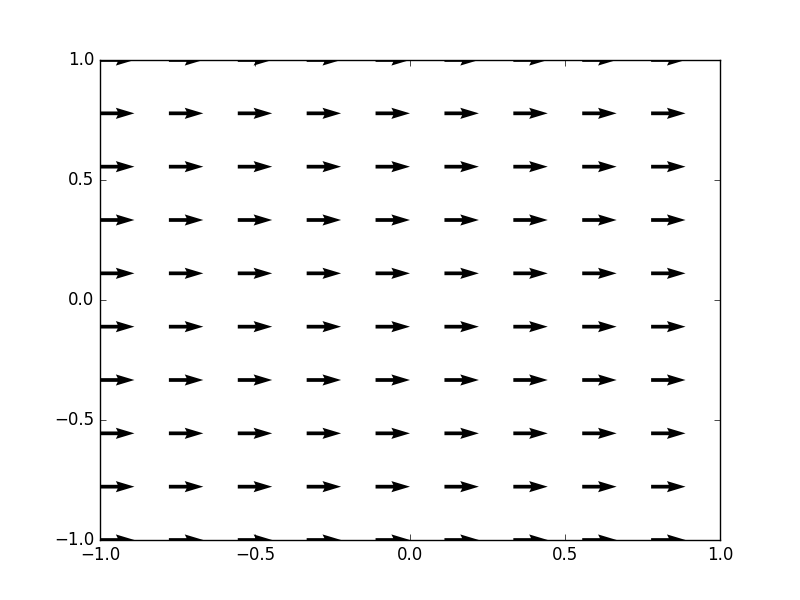
\includegraphics[width=\textwidth]{qplate(0).png}
			\caption{$q=0$, $\alpha_0=0$}
			\label{fig:q0}
		\end{subfigure}
		\hfil
		\begin{subfigure}[H]{0.35\textwidth}
			\centering
			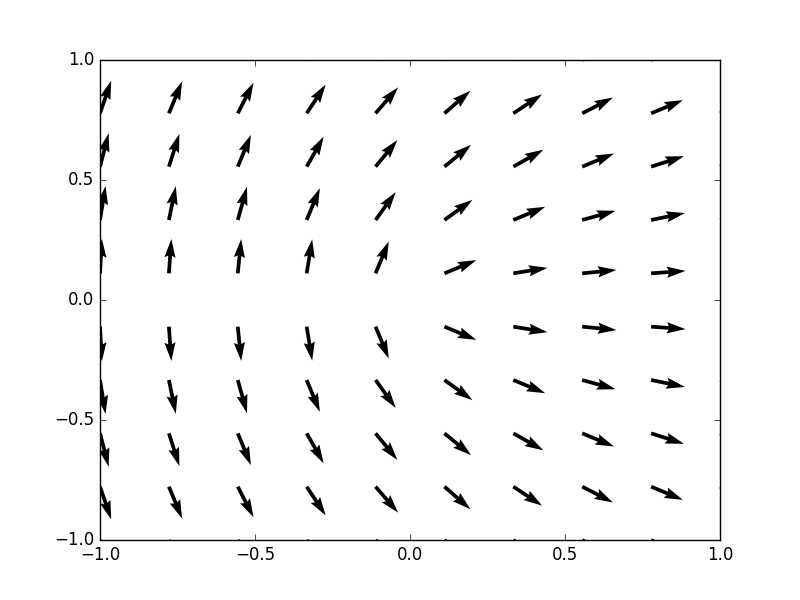
\includegraphics[width=\textwidth]{qplate(0.5).png}
			\caption{$q=0.5$, $\alpha_0=0$}
			\label{fig:q0.5}
		\end{subfigure}
	\end{figure}
	\begin{figure}[H]
		\begin{subfigure}[H]{0.35\textwidth}
			\centering
			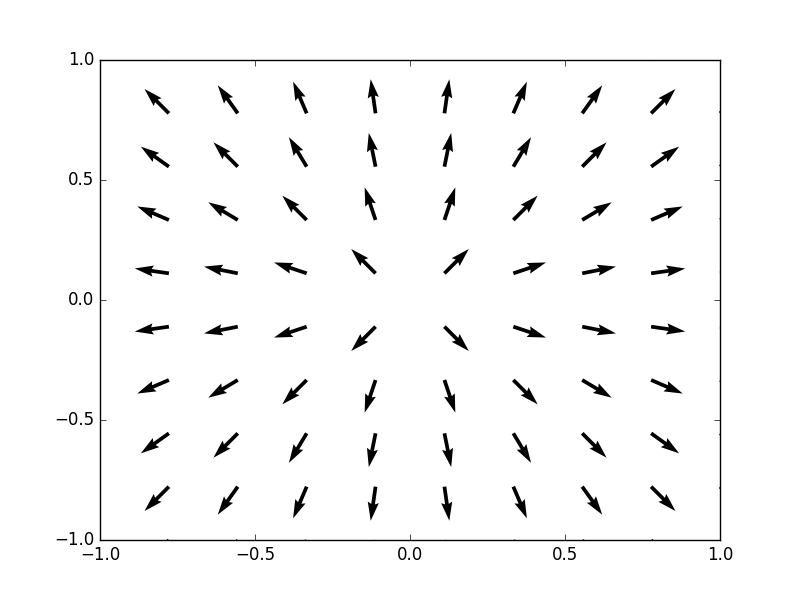
\includegraphics[width=\textwidth]{qplate(1).png}
			\caption{$q=1$, $\alpha_0=0$}
			\label{fig:q1}
		\end{subfigure}
		\hfil
		\begin{subfigure}[H]{0.35\textwidth}
			\centering
			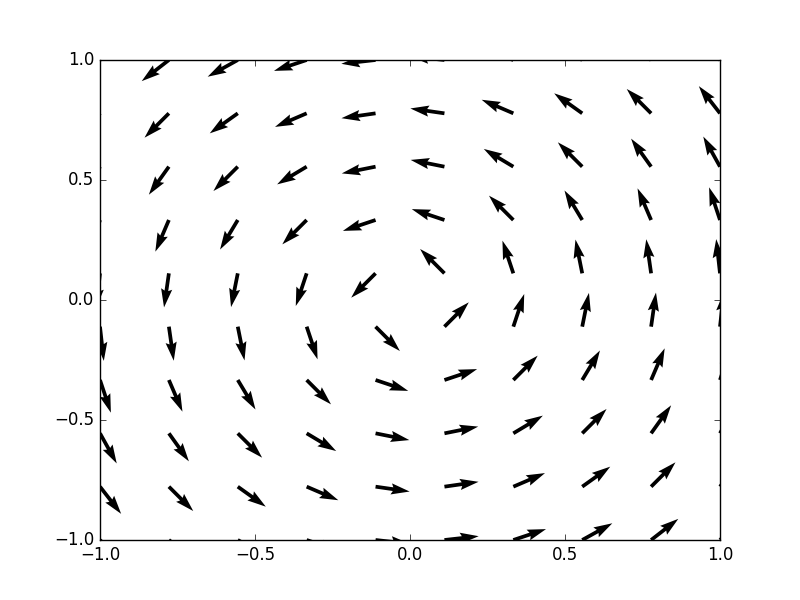
\includegraphics[width=\textwidth]{qplate(1,r).png}
			\caption{$q=1$, $\alpha_0=\pi/2$}
			\label{fig:q1r}
		\end{subfigure}
	\end{figure}
\end{frame}

\begin{frame}{SOI in q-plate}\blfootnote{Marrucci, L. (2006), Wave Optics (2015)}
	\textbf{Q-plate of phase retardation of $\pi$}
	\begin{align*}
		\onslide<2->{
		\begin{bmatrix}
			1\\i\sigma
		\end{bmatrix}
		\longrightarrow\;
		&\boxed{\textbf{\text{Q}}_{\lambda/2}}\;\longrightarrow}
		\onslide<3->{
		\begin{bmatrix}
			1\\-i\sigma
		\end{bmatrix}
		\alert{\underbrace{\exp(i2\sigma q\phi)}_{\text{Vortex}}}
		\:\exp(i2\sigma\alpha_0)}\\
		\onslide<4->{(\sigma=\pm1,l=0) &\longrightarrow (\sigma=\mp1,l=\pm\alert{2q})}
	\end{align*}
	\onslide<5>{$q=1\rightarrow$ Angular momentum per photon is conserved.}
	\onslide<6->{\textbf{Q-plate of phase retardation of $\pi/2$}}
	\begin{align*}
		\onslide<7->{
			\begin{bmatrix}
				1\\i\sigma
			\end{bmatrix}
			\longrightarrow\;
			&\boxed{\textbf{\text{Q}}_{\lambda/4}}\;\longrightarrow}
		\onslide<8->{
			\begin{bmatrix}
				\cos(\alpha - \sigma\pi/4)\\
				\sin(\alpha - \sigma\pi/4)
			\end{bmatrix}
			\alert{\underbrace{\exp(i\sigma q\phi)}_{\text{Vortex}}}
			\:\exp(i\sigma\alpha_0)}\\
		\onslide<9->{(\sigma=\pm1,l=0) &\longrightarrow (\sigma=0,l=\pm\alert{q})}
	\end{align*}
	\onslide<10>{$q=1\rightarrow$ Angular momentum per photon is conserved.}
\end{frame}

\begin{frame} %thanks
	\begin{center}\Huge
		\alert{THANKS\\
		TO ALL}
	\end{center}
\end{frame}
\end{document}